\documentclass{article}
\usepackage[utf8]{inputenc}
\usepackage[margin=1in]{geometry}
\usepackage{setspace,mathtools,indentfirst,hyperref,graphicx,listings,courier,color}
\usepackage{float}

\doublespacing{}

\lstset{%
  basicstyle=\ttfamily,
  captionpos=b,
  frame=tb,
  tabsize=2,
  showstringspaces=false,
  commentstyle=\color[RGB]{24,135,64},
  keywordstyle=\color{blue},
  stringstyle=\color{red}
}
\begin{document}
\noindent Nelson Batista, Max Inciong, and Francesca Truncale

\noindent Senior Project II --- Fall 2017

\noindent Professor Jianting Zhang

\noindent Report for Oct. 10

This week, we completed almost the entirety of the CPU implementation. The only remaining tweak is to modify the \texttt{find\_isomorphism} function to return the \textit{number} of matches of the subgraph in the larger graph, rather than simply whether there is a match. We are currently debugging this particular modification, and it should be complete by the middle of this week.

We have looked into timing considerations, and used Python's built-in profiling tools to analyze the performance of the CPU code. On the Facebook graph we are using, finding a single instance of subgraph isomorphism takes around 12-15 seconds. Below is the result of one sample run.

\begin{figure}[H]
  \centering
  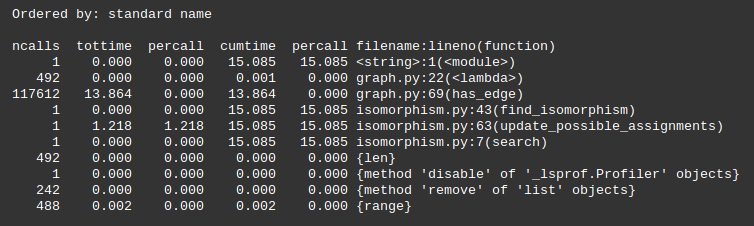
\includegraphics[scale=0.6]{perf}
  \caption{Sample run of the CPU implementation of subgraph isomorphism.}
\end{figure}

We see that the overwhelming majority of the time is spent calling the \texttt{has\_edge} method of the graph class. This method, shown below, calls the built-in \texttt{in} function of Python lists. 

\lstinputlisting[language=Python,firstline=69,lastline=72,caption={\texttt{has\_edge} method of our graph class.}]{../../src/pythonvers/graph.py}

This method has a runtime complexity of O(n) (see the table at \url{https://wiki.python.org/moin/TimeComplexity}), and is called \textit{117,612} times in the sample run. This is an obscene number of calls, and is adequately explained by looking at the \texttt{update\_possible\_assignments} function, called by \texttt{find\_isomorphism}:

\lstinputlisting[language=Python,firstline=71,caption={Contents of the \texttt{update\_possible\_assignments} function.}]{../../src/pythonvers/isomorphism.py}

We see that \texttt{has\_edge} is called once per each iteration of the innermost loop, which runs for as many iterations as the graph has vertices (which is many if the graph is large, as ours is), which is itself contained within another for loop with many iterations. Suffice to say, the algorithm's performance would benefit greatly from being able to parallelize this particular loop, since it gets called so many times.

\end{document}
